\vspace{-10pt}
\section{Experimental evaluation}
\vspace{-5pt}
We evaluate the performance of FlashMatrix on statistics and machine learning
algorithms both in memory and on SSDs. We compare their performance with
the implementations in Spark MLlib \cite{mllib}, a highly-optimized parallel
machine learning library, and the C and FORTRAN implementations in the R framework.

%We further illustrate the effectiveness of the optimizations deployed in
%FlashMatrix when running both in memory and on SSDs.

We conduct experiments on a NUMA machine with
four Intel Xeon E7-4860 2.6 GHz processors and 1TB of 
DDR3-1600 memory. Each processor has 12 cores. The machine has three LSI SAS 9300-8e
host bus adapters connected to
24 OCZ Intrepid 3000 SSDs. The SSDs are capable of
12 GB/s for read and 10 GB/s for write. The machine runs
Linux kernel v3.13.0. By default, we use 48 threads. 
We use Spark v1.5.0 and R v3.2.4.

%\subsection{Statistics and Machine learning algorithms} \label{sec:apps}

Using the R interface of FlashMatrix, we implement the algorithms of 
Table \ref{tbl:algs}, using the same algorithmic approach as MLlib.
The two clustering algorithms 
K-means \cite{kmeans} and Gaussian Mixture Model (GMM) \cite{gmm} 
were recognized as top 10 data mining algorithms \cite{top10}. 
Singular value decomposition (SVD) is the canonical approach to 
reducing dimension based on eigensolving.  Correlation 
(pair-wise Pearson's correlation \cite{cor}) is commonly used in statistics.
Summary computes a suite of multivariate statistics:
column-wise minimum, maximum, mean, L1 norm, L2 norm, number of non-zero values and
		variance.
Algorithms exhibit various ratios of computation to I/O, which aids
a thorough evaluation.
%hich helps to evaluate perforamnce %of FlashMatrix
%on SSDs 
%thoroughly. 



%We implement multiple important algorithms in the field of statistics and
%machine learning. We implement these
%algorithms completely with the R interface of FlashMatrix and
%rely on FlashMatrix to perform computation in parallel and out of core.
%\begin{itemize}
%	\item 
%
%\para{Multivariate statistical summary} 
%column-wise minimum,
%		maximum, mean, L1 norm, L2 norm, the number of non-zero values and
%		variance.
%
%%	\item 
%\para{Correlation} pair-wise Pearson's correlation \cite{cor}
%		among multiple series is commonly used in statistics.
%
%\para{Singular value decomposition (SVD)} factors a matrix into
%		three matrices: $U$, $\Sigma$ and $V$ such that $A=U \Sigma V^T$, where
%		$U$ and $V$ are orthonormal matrices and $\Sigma$ is a diagonal
%		matrix with non-negative diagonals in descending order. 
%%To compute SVD
%%		on a $n \times p$ matrix $A$ ($n \gg p$), we first compute Gramian
%%		matrix $A^T A$ and compute eigenvalues and eigenvectors to derive singular
%%		values and singular vectors of the matrix $A$. 
%SVD is commonly used for dimension reduction. 
%%In the experiments, we compute 10 singular values.
%%
%\para{K-means \cite{kmeans}} an iterative algorithm that partitions 
%%		data points into $k$ clusters so that each cluster has minimal mean
%		of distances between the data points and the cluster center. 
%%K-means
%%		is one of the most popular clustering algorithms and 
%is one of the top 10 data mining algorithms \cite{top10}. 
%In the experiments, we run k-means to split a dataset into 10 clusters by default.

%\para{Gaussian Mixture Model (GMM) \cite{gmm}} an iterative clustering
%		algorithm 
%%that assumes data points are sampled from a mixture of
%%		Gaussian distributions and 
%  that use expectation maximization (EM)
%		to fit data to Gaussian distributions. This is also one
%		of the top 10 data mining algorithms \cite{top10}. 
%%In the experiments, we run GMM to split a dataset into 10 clusters by default.
%%:\end{itemize}
%
\begin{table}
\begin{center}
\footnotesize
\begin{tabular}{|c|c|c|c|c|}
\hline
Algorithm & Computation & I/O \\
\hline
Summary & $O(n \times p)$ & $O(n \times p)$ \\
\hline
Correlation & $O(n \times p^2)$ & $O(n \times p)$ \\
\hline
SVD & $O(n \times p^2)$ & $O(n \times p)$ \\
\hline
K-means (1 iteration) & $O(n \times p \times k)$ & $O(n \times p)$ \\
\hline
GMM (1 iteration) & $O(n \times p^2 \times k + p^3 \times k)$ & $O(n \times p + n \times k)$ \\
\hline
\end{tabular}
\normalsize
\end{center}
\vspace{-10pt}
\caption{Computation and I/O complexity. 
$n$ is the number of data points, $p$ 
is the number of the features in a point, and $k$ is the number of
clusters. }
\label{tbl:algs}
\end{table}

%These algorithms have various ratios of computation complexity and I/O complexity
%(Table \ref{tbl:algs}), which helps to evaluate perforamnce %of FlashMatrix
%%on SSDs 
%thoroughly. 
%The first three algorithms require a constant number
%of passes over the input matrix. K-means and GMM run iteratively and we show
%their computation and I/O complexity in a single iteration. GMM typically run
%on a dataset with a small number of features. Therefore, the first term of its
%computation complexity dominates the computation. Although correlation and SVD
%have lower asymptotic complexity than GMM, they may run on datasets with many
%features and, thus, may have very high computation overhead.

\begin{table}
\begin{center}
\footnotesize
\begin{tabular}{|c|c|c|c|c|}
\hline
Data Matrix & n & p & size \\
\hline
Friendster-32 \cite{friendster} & 65M & 32 & 16GB \\
\hline
MixGaussian-1B & 1B & 32 & 251GB \\
\hline
Random-65M & 65M & 8-512 & 4-248GB \\
\hline
\end{tabular}
\normalsize
\end{center}
\vspace{-10pt}
\caption{Datasets ($n \times p$ matrices).}
\label{tbl:data}
\vspace{-10pt}
\end{table}

K-means and GMM typically run on a dataset with a small number of features
in each data point, owing to curse of dimensionality \cite{Jain00}.
% while
%the other algorithms may be applied to datasets with various numbers of
%features.
We run k-means and GMM on
the Friendster-32 matrix, constructed from 32 eigenvectors of the Friendster
graph \cite{friendster}, as well as the MixGaussian-1B
sampled from 10 mixtures of multivariate Gaussian distributions.
The other algorithms run on all matrices (Table \ref{tbl:data}),
including random matrices with 65 million rows and columns
varying from 8 to 512.

%data points and 32 features in each data point.
%
% We use the datasets in Table \ref{tbl:data} for performance
%evaluation. In all datasets, the number of data points is far more than
%the number of features. 

%with the identity covariance matrix and different means. 

%\vspace{-8pt}
%\subsection{Comparative performance}
%\vspace{-4pt}
\para{Comparative performance}
We evaluate FlashMatrix against
Spark MLlib \cite{mllib} and R. We run the MLlib algorithms
with their native Scala interface and use a large heap size to ensure that
all data are cached in memory. We use 48 threads for both FlashMatrix and
MLlib. %to run on the MixGaussian-1B matrix.
The R framework provides C implementations for correlation, SVD and k-means.
The R package mclust \cite{mclust} provides a FORTRAN implementation of GMM.
%These implementations run in a single thread. We run the FlashMatrix
%implementations in a single thread and compare their performance with the C and
%FORTRAN implementations on the Friendster-32 matrix.

\begin{figure}
  \vspace{-5pt}
	\centering
	\footnotesize
	\begin{subfigure}{.5\textwidth}
		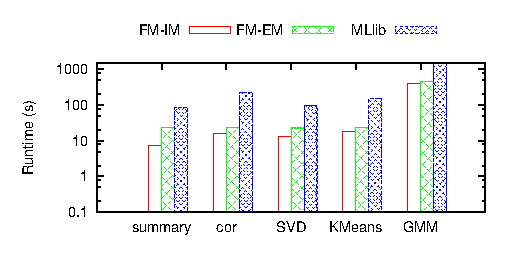
\includegraphics{FlashMatrix_figs/FM-vs-spark.eps}
		\label{perf:rt}
		\vspace{-12pt}
		\caption{Runtime}
	\end{subfigure}

	\vspace{3pt}
	\begin{subfigure}{.5\textwidth}
		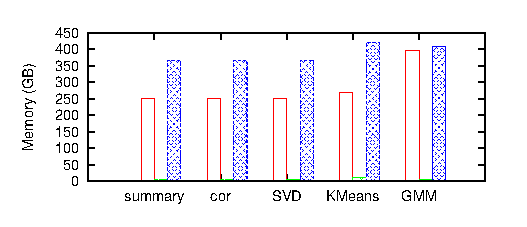
\includegraphics{FlashMatrix_figs/FM-vs-spark-mem.eps}
		\label{perf:mem}
		\vspace{-12pt}
		\caption{Memory consumption}
	\end{subfigure}
	\caption{The performance and memory consumption of FlashMatrix both
		in memory (FM-IM) and on SSDs (FM-EM) compared with Spark MLlib
		on the MixGaussian-1B matrix.}
	\label{perf:fm}
  \vspace{-10pt}
\end{figure}

FlashMatrix outperforms Spark MLlib significantly
on all algorithms (Figure \ref{perf:fm}(a)). For 
correlation, SVD and GMM, both FlashMatrix and MLlib
rely on BLAS for matrix multiplication; the differences lie in memory access.
MLlib materializes operations such as aggregation separately and implements
non-BLAS operations with Scala. The matrix fusion and materialization of
two-level partitioning of FlashMatrix result in a 3 to 10 times performance
gain when compared with MLlib.

% FlashMatrix outperforms MLlib significantly owing to our heavy optimizations on GenOps
%such as aggressive matrix operation fusion and VEleFuns. In contrast, 
%SVD is the only application whose FlashMatrix
%implementation does not outperform the one in MLlib when being executed out of
%core because this application requires to read the entire matrix multiple times
%and output a large matrix.

%Even though FlashMatrix provides a matrix-oriented functional programming
%interface, it 
FlashMatrix easily scales to datasets with billions of data points
(Figure \ref{perf:fm}(b)) and uses negligible amounts of memory when running out-of-core.
%. Its
%scalability is bound by the capacity of SSDs 
%For out-of-core execution, FlashMatrix keeps large matrices on
%SSDs.  % and has a very small memory footprint.  
Lazy evaluation and virtual matrices make it so that data are streamed from 
inputs to outputs with SSD I/O.  Memory consumption is below 10 GB for all inputs.
%We did not encounter the scalability limits of FlashMatirx
%We have not found the scalability limits of out-of-core FlashMatrix, but it will not be 
%from running out of memory.
%The functional programming
%interface generates a new matrix in each matrix operation, which potentially
%leads to high memory consumption. 
%Owing to lazy evaluation, FlashMatrix does not store majority of matrices in the computation physically.
%As such, its in-memory 
%out-of-core execution barely increases memory consumption from
%the minimum memory requirement of the algorithms. 
%This indicates that the out-of-core execution consumes small space on SSDs, which leads to
%very high scalability.

FlashMatrix running both in memory and on SSDs significantly outperforms R
(Figure \ref{fig:fmR}).  Because R's implementations are single threaded,
we run FlashMatrix in a single thread. 
%for all algorithms even with a single thread in all of these algorithms 
We exclude ``Summary'' because R does not provide an implementation for
the same statistics.
%a C or FORTRAN implementation of computing the same statistics. 
%The performance
%results indicate that FlashMatrix executes R code efficiently to even outperform
%some optimized C and FORTRAN implementations when processing large datasets.

\begin{figure}[b]
  \vspace{-10pt}
	\begin{center}
		\footnotesize
		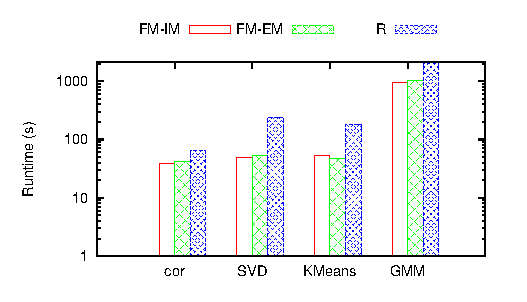
\includegraphics{FlashMatrix_figs/FM-vs-R.eps}
		\caption{In-memory (FM-IM) and out-of-fore (FM-EM) FlashMatrix 
        in a single thread compared with R's C and FORTRAN implementations on Friendster-32.}
		\label{fig:fmR}
	\end{center}
  \vspace{-15pt}
\end{figure}

\begin{comment}
\begin{figure}
	\begin{center}
		\footnotesize
		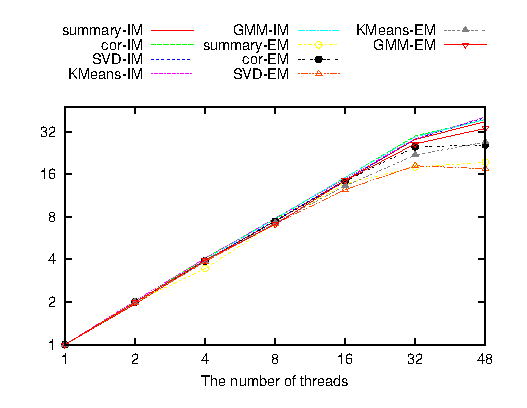
\includegraphics{FlashMatrix_figs/speedup.eps}
		\caption{The speedup of FlashMatrix with multithreading both in memory (IM)
		and on SSDs (EM).}
		\label{fig:speedup}
	\end{center}
\end{figure}

In-memory FlashMatrix achieves near linear speedup whereas the out-of-core execution 
starts to flatten after 32 threads (Figure \ref{fig:speedup}).
Operation fusion and reducing data movement removes memory bandwidth bottlenecks, allowing 
scaling with more CPU cores. 
% . As such, memory bandwidth is no longer the bottleneck
%for in-memory execution and the algorithms speed up linearly with more CPU cores.
Out-of-core, I/O becomes the bottleneck for the algorithms with
lower computation complexity. However,
GMM still speeds up almost linearly even when running on SSDs, due to its high
computation complexity. The performance results in Figure \ref{fig:fmR} and Figure
\ref{fig:speedup} indicate that FlashMatrix can potentially execute R code with
performance comparable to parallel C or FORTRAN implementations.
\end{comment}

%\vspace{-8pt}
%\subsection{Out-of-core v. in-memory performance}
%\vspace{-4pt}
\para{Out-of-core versus in-memory performance}
We further compare the in-memory and external-memory performance of FlashMatrix.
%thoroughly with different datasets and different parameters. 
We run the first three algorithms on random-65M matrices
with the number of columns varying from 8 to 512. We run k-means
and GMM on the Friendster-32 matrix and vary the number of clusters from 2 to 64.

\begin{figure}[t]
	\begin{center}
		\footnotesize
		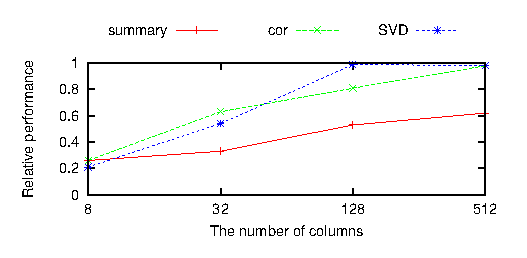
\includegraphics{FlashMatrix_figs/IM-vs-EM-stat.eps}
		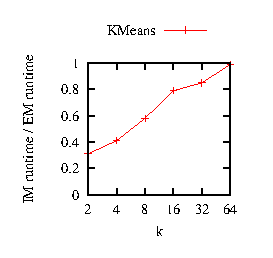
\includegraphics{FlashMatrix_figs/IM-vs-EM-clust.eps}
		\caption{{\em FlashMatrix} scaleup: The performance on SSDs  (FM-EM)
      normalized to in-memory performance (FM-IM) on random-65M 
      while varying the number of columns (top) and for
clustering algorithms while varying the number of clusters (bottom).}
%normalized by its performance
%			in memory. 
%      As the number of columns increases, performance out-of-core
%			approaches in-memory performance.}
		\label{perf:stat}
	\end{center}
  \vspace{-15pt}
\end{figure}

As the number of features or clusters increases,
the performance gap between in-memory and external-memory execution
narrows and the external-memory performance approaches 
in-memory performance for all algorithms but Summary (Figure \ref{perf:stat}).
% and \ref{perf:clust}).
This observation conforms with the computation and I/O complexity of
the algorithms in Table \ref{tbl:algs}.
For Correlation, SVD, k-means, and GMM, the number of clusters or features causes computation
to grow more quickly than the I/O, driving performance toward a compute bound.
% When the number of features
%gets larger, the computation of matrix multiplication in
%correlation and SVD grows more rapidly than I/O and eventually CPU becomes
%the bottleneck. The current implementation of correlation requires an additional
%pass on the input matrix to compute column-wise mean values, which results in
%lower external-memory performance. Similarly, as the number of clusters
%increases, the computation of k-means and GMM increases rapidly and
%these algorithms are dominated by their CPU computation as the number
%of clusters gets larger. 
The compute bound can be realized on few features or clusters for an I/O throughput of 10GB/s.
%Given an I/O throughput of 10 GB/s, the algorithms
%do not require many features or clusters to have their external-memory
%performance close to their in-memory performance.

%\begin{figure}
%	\begin{center}
%		\footnotesize
%		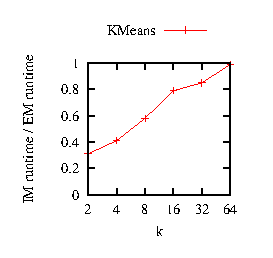
\includegraphics{FlashMatrix_figs/IM-vs-EM-clust.eps}
%		\caption{{\em Clustering} scaleup: FlashMatrix performance on SSDs 
%      normalized to in-memory performance as the number of clusters vary. 
%%      KMeans operates on the \rb{Friendster32} matrix and GMM on the  
%%			by its performance in memory. As the number of clusters increases,
%%			the external-memory performance of these implementations approach
%%			to their in-memory performance.}
%}
%		\label{perf:clust}
%	\end{center}
%\end{figure}

%\vspace{-8pt}
%\subsection{Effectiveness of optimizations}
%\vspace{-4pt}
\para{Effectiveness of optimizations}
We illustrate the effectiveness of our memory optimizations in FlashMatrix.
We focus on two main optimizations: matrix operation fusion in main memory
to reduce data movement between SSDs and main memory (mem-fuse), and matrix
operation fusion in CPU cache to reduce data movement between main memory and
CPU cache (cache-fuse).

Both optimizations have significant performance improvement on all
algorithms when FlashMatrix runs on SSDs (Figure \ref{perf:em_opts}).
Operation fusion in main memory (mem-fuse) achieves
substantial performance improvement in most algorithms, even in GMM,
which has the highest asymptotic computation complexity. 
%Even though the SSDs deliver an I/O throughput of 10GB/s, 
Materializing every matrix operation
separately causes SSDs to be the main bottleneck in the system and
fusing matrix operations in memory significantly reduces I/O.
% and improves performance by a large factor. 
Operation fusion in the CPU cache (cache-fuse) doubles or even triples
performance in some of the algorithms,
which suggests that memory bandwidth is a limiting performance factor once 
I/O has been optimized.
 %This suggests that with sufficient 
%I/O optimizations, many machine learning algorithms that run on fast SSDs can be bottlenecked by
%the bandwidth of main memory, instead of I/O. 
%Even though it is less noticeable,
%Finally, reducing large memory allocation (mem-alloc) improves I/O performance and almost doubles
%the overall performance of all algorithms.

\begin{figure}
	\begin{center}
		\footnotesize
		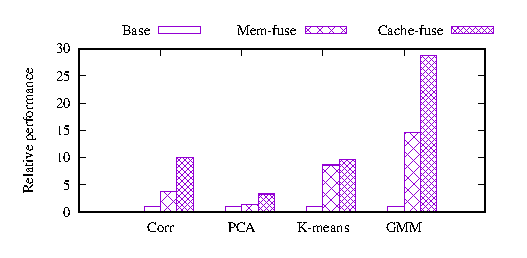
\includegraphics{FlashMatrix_figs/opts-EM.eps}
		\vspace{-10pt}
		\caption{The effectiveness of optimizations on different algorithms
		running on SSDs. The optimizations are applied to FlashMatrix
		incrementally.}
		\label{perf:em_opts}
	\end{center}
  \vspace{-15pt}
\end{figure}
